\documentclass[aspectratio=169]{beamer}


\usepackage[utf8]{inputenc}
\usepackage{amsmath}
\usepackage{amsfonts}
\usepackage{amssymb}
\usepackage{xcolor}
\usepackage{graphicx}
\usepackage{ragged2e}  % `\justifying` text
\usepackage{booktabs}  % Tables
\usepackage{tabularx}
\usepackage{tikz}      % Diagrams
\usetikzlibrary{calc, shapes, backgrounds}
\usepackage{amsmath}
\usepackage{amssymb}
\usepackage{dsfont}
\usepackage{url, soul}       % `\url
\usepackage{listings}  % Code listings
\usepackage[T1]{fontenc}
\usepackage{theme/beamerthemehbrs}

\author[Veeramacheneni]{Lokesh Veeramacheneni}
\title{Out-of-Distribution Detection in 3D Semantic Segmentation}
\subtitle{Master Thesis}
\institute[HBRS]{Hochschule Bonn-Rhein-Sieg}
\date{September 02, 2022}
\subject{Test beamer}

% leave the value of this argument empty if the advisors
% should not be included on the title slide
\def\advisors{Prof. Dr. Paul G Pl\"{o}ger, Prof. Dr. Matias Valdenegro Toro, Prof. Dr. Sebastian Houben}

\thirdpartylogo{images/DFKI.png}


\begin{document}
{
\begin{frame}
\titlepage
\end{frame}
}

%%%%%%%%%%%%%%%%%%%%%%%%%%%%%%%%%%%%%%%%%%%%%%%%%%%%%%%%%%%%%%%%%%%%%%%%%%%%%%%%%%%%%%%%
%%%%%%%%%%%%%%%%%%%%%%%        Introduction           %%%%%%%%%%%%%%%%%%%%%%%%%%%%%%%%%%
%%%%%%%%%%%%%%%%%%%%%%%%%%%%%%%%%%%%%%%%%%%%%%%%%%%%%%%%%%%%%%%%%%%%%%%%%%%%%%%%%%%%%%%%
\section{Introduction}
% 1. Discuss about what is OOD
% and need for OOD along with some real life examples
% 2. Explain about 3D Semantic segmentation task
\begin{frame}{Out-of-Distribution detection}
    \begin{itemize}
        \item An ideal trustworthy visual recognition system
        \begin{itemize}
            \item Produce accurate predictions on known examples
            \item Detect and reject unknown examples
        \end{itemize}
        \item Deep Neural Networks (DNNs) are trained based on closed world assumption
        \item closed world assumption - test data is assumed to be drawn from same distribution as training data which is called In-Distribution (ID)
        \item When deployed in real world (open world scenario) the test samples can be Out-of-Distribution (OOD) i.e. the test samples can be,
        \begin{itemize}
            \item from different class
            \item from different domain 
        \end{itemize}
    \end{itemize}
\end{frame}
\begin{frame}{Out-of-Distribution detection}
 \begin{columns}
    \begin{column}{0.5\textwidth}
        \begin{itemize}
            \item A real world example for OOD object is described in Figure~\ref{fig:eg_tesla_moon}
            \item Tesla autonomous driving system detects the moon as the yellow traffic light
            \item These faulty predictions might result in output of the autonomous driving system being catastrophic
        \end{itemize}
    \end{column}
    \begin{column}{0.5\textwidth}
     \begin{figure}
         \centering
         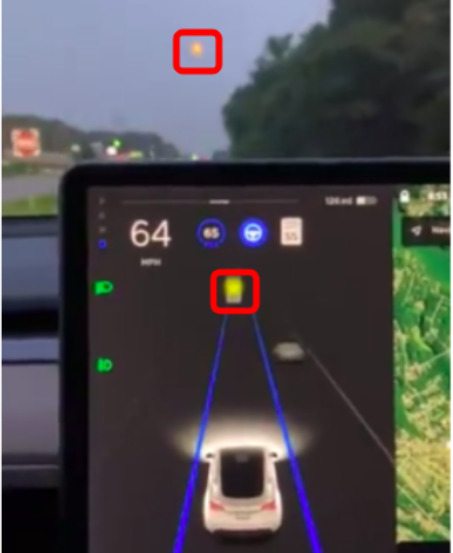
\includegraphics[scale=0.25]{images/Tesla_ex_moon.jpg}
         \caption{Caption}
         \label{fig:eg_tesla_moon}
     \end{figure}
    \end{column}
 \end{columns}
\end{frame}
\begin{frame}{Importance of OOD detection}
    \begin{columns}
       \begin{column}{0.5\textwidth}
        \begin{itemize}
            \item Figure~\ref{fig:eg_apollo_pipeline} depicts the pipeline of modules in Apollo driving platform.
            \item Prediction and motion planning module are dependent on perception module.
            \item A misdetection of an OOD sample will propogate the error to motion planning and affects the total vehicle control and this might lead to unfortunate consequence
        \end{itemize}
       \end{column}
       \begin{column}{0.5\textwidth}
            \begin{figure}
                \centering
                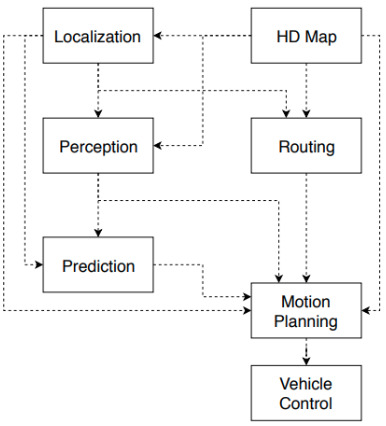
\includegraphics[scale=0.35]{images/apollo_pipeline.jpg}
                \caption{Caption}
                \label{fig:eg_apollo_pipeline}
            \end{figure}
       \end{column}
    \end{columns}
\end{frame}
\begin{frame}{3D Light Detection And Ranging (LiDAR)}
    \begin{columns}
       \begin{column}{0.5\textwidth}
            \begin{itemize}
                \item Uses pulsed lasers to find the range to the objects
                \item Unlike images, LiDAR is insusceptible to illumination and provide rich 3D information.
                \item Figure~\ref{fig:sample_lidar_pc} depicts the sample point cloud with LiDAR is placed in round white circle found at the center of point cloud
                \item Typically, features of each point in point cloud include 
                \begin{itemize}
                    \item spatial features (XYZ)
                    \item Colour (RGB)
                    \item Intensity
                \end{itemize}
            \end{itemize}
       \end{column}
       \begin{column}{0.5\textwidth}
            \begin{figure}
                \centering
                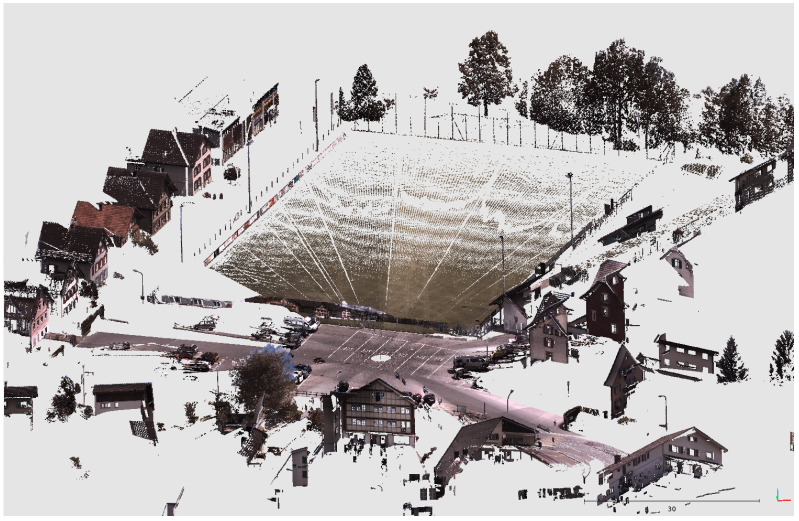
\includegraphics[scale=0.25]{images/sample_LiDAR_PC.jpg}
                \caption{Caption}
                \label{fig:sample_lidar_pc}
            \end{figure}
       \end{column}
    \end{columns}
\end{frame}
\begin{frame}{3D Semantic Segmentation}
    \begin{columns}
       \begin{column}{0.4\textwidth}
            \begin{itemize}
                \item An important task in computer vision because of its use in scene understanding
                \item Further helps in navigation and planning of robots
                \item Objective - Assign each point in the point cloud a specific class
            \end{itemize}       
       \end{column}
       \begin{column}{0.6\textwidth}
            \begin{figure}
                \centering
                %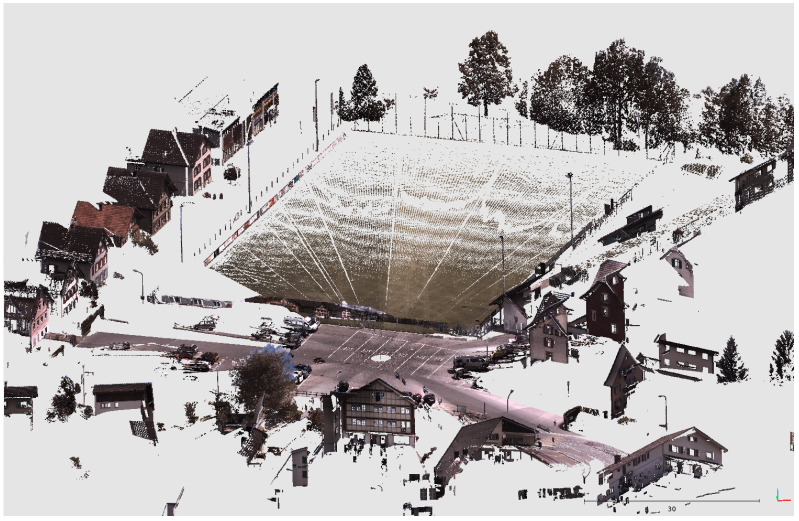
\includegraphics[scale=0.15]{images/sample_LiDAR_PC.jpg}
                %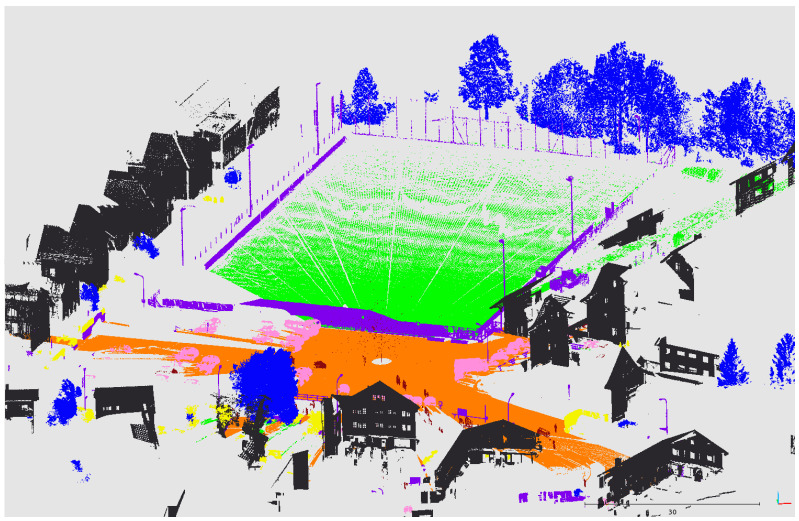
\includegraphics[scale=0.15]{images/sample_LiDAR_PC_segmented.jpg}
                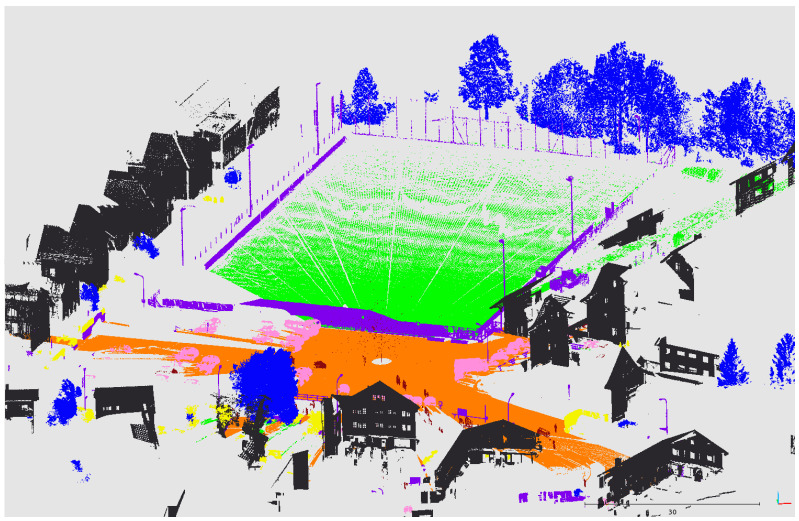
\includegraphics[scale=0.3]{images/sample_LiDAR_PC_segmented.jpg}
                \caption{Caption}
                \label{fig:sample_lidar_pc_segmented}
            \end{figure}
       \end{column}
    \end{columns}
\end{frame}

\begin{frame}{Thesis objective}

\begin{itemize}
    \item OOD detection in the 3D semantic segmentation setting
    \item Create a benchmark datasets for OOD detection among existing 3D LiDAR datasets. We define OOD data based on two categories
    \begin{itemize}
        \item if the point is from different class than training data
        \item if the point has inferior quality
    \end{itemize}
    \item We also study whether uncertainty estimation is a practical approach for OOD detection in 3D domain
\end{itemize}
    
\end{frame}
%%%%%%%%%%%%%%%%%%%%%%%%%%%%%%%%%%%%%%%%%%%%%%%%%%%%%%%%%%%%%%%%%%%%%%%%%%%%%%%%%%%%%%%%
%%%%%%%%%%%%%%%%%%%%%%%        Methodology           %%%%%%%%%%%%%%%%%%%%%%%%%%%%%%%%%%%
%%%%%%%%%%%%%%%%%%%%%%%%%%%%%%%%%%%%%%%%%%%%%%%%%%%%%%%%%%%%%%%%%%%%%%%%%%%%%%%%%%%%%%%%
\section{Methodology}
% Explain about what are the requirements for setup one by one such as
% Datasets & benchmarking, OOD method, 3D Model, Uncertainty methods, Evaluation metrics
\begin{frame}{Ingredients}
    \begin{itemize}
        \item Datasets
        \item 3D Semantic Segmentation model
        \item Uncertainty methods
        \item OOD score methods
    \end{itemize}
\end{frame}
\begin{frame}{3D LiDAR datasets}
    \begin{figure}
        \centering
        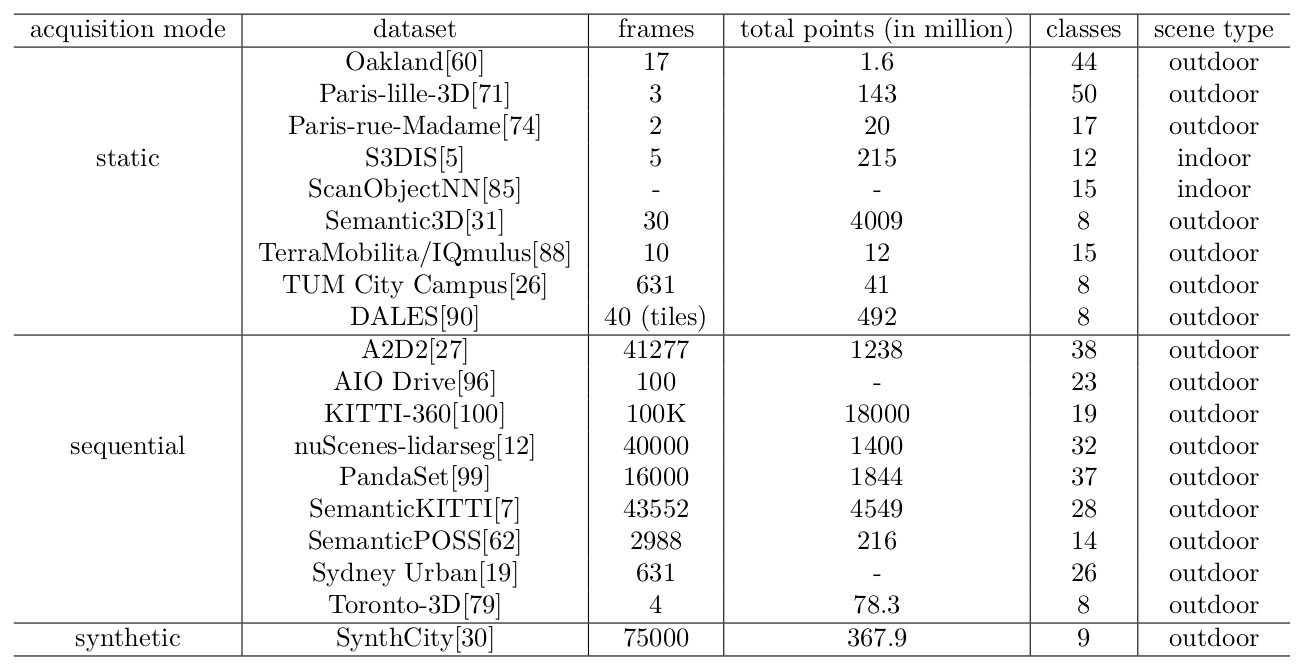
\includegraphics[scale=0.25]{images/3d_datasets.jpg}
        \caption{caption}
        \label{fig:datasets}
    \end{figure}
\end{frame}
\begin{frame}{Semantic3D}
    \begin{columns}
        \begin{column}{0.5\textwidth}
            \begin{itemize}
                \item Huge 3D point cloud benchmark classification static dataset with 4 million points
                \item Scenes are taken in european streets around church, stations and fields
                \item Point features include XYZ, RGB and Intensity values.
                \item It has 8 classes with distribution of points represented in Figure\ref{fig:sem3d_stats}
                \item cite states that the scanning artefacts, hardscapes and cars are the most challenging classes
            \end{itemize}
        \end{column}
        \begin{column}{0.5\textwidth}
            \begin{figure}
                \centering
                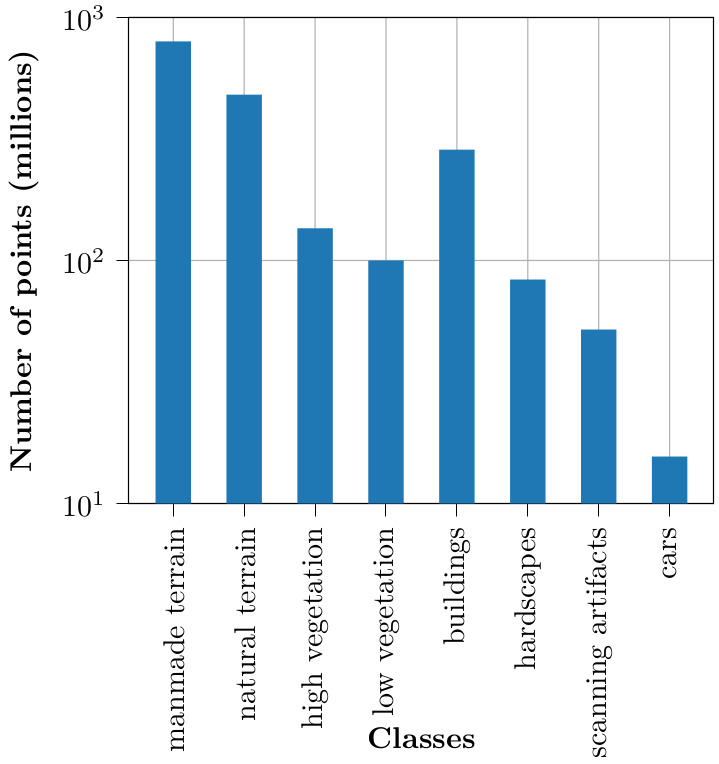
\includegraphics[scale=0.25]{images/sem3d/sem3d_stats.jpg}
                \caption{caption}
                \label{fig:sem3d_stats}
            \end{figure}
        \end{column}
    \end{columns}
\end{frame}
\begin{frame}{Semantic3D}
    \begin{columns}
        \begin{column}{0.33\textwidth}
            \begin{figure}
                \centering
                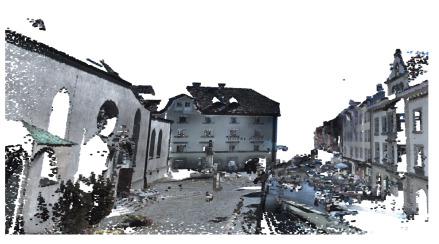
\includegraphics[scale=0.33]{images/sem3d/sem3d_sample_1.jpg}
                %\caption{caption}
                %\label{fig:sem3d_sample_1}    
            \end{figure}
        \end{column}
        \begin{column}{0.33\textwidth}
            \begin{figure}
                \centering
                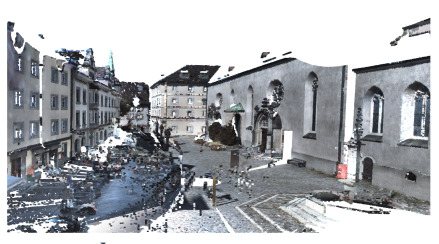
\includegraphics[scale=0.33]{images/sem3d/sem3d_sample_2.jpg}
                \caption{caption}
                \label{fig:sem3d_sample_2}    
            \end{figure}
        \end{column}
        \begin{column}{0.33\textwidth}
            \begin{figure}
                \centering
                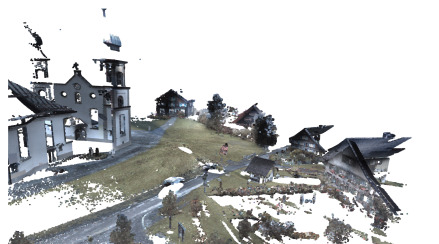
\includegraphics[scale=0.33]{images/sem3d/sem3d_sample_3.jpg}
                %\caption{caption}
                %\label{fig:sem3d_sample_3}    
            \end{figure}
        \end{column}
    \end{columns}
\end{frame}
\begin{frame}{S3DIS}
    \begin{columns}
        \begin{column}{0.6\textwidth}
            \begin{itemize}
                \item Indoor dataset with scans from various buildings
                \item Dataset include scans of personal offices, restrooms, open spaces, lobbies and hallways
                \item It has 12 classes, further subdivided into two types
                \begin{itemize}
                    \item structural elements 
                    \item everyday items
                \end{itemize}
                \item One of the most evaluated datasets for indoor semantic segmentation
            \end{itemize}
        \end{column}
        \begin{column}{0.4\textwidth}
            \begin{figure}
                \centering
                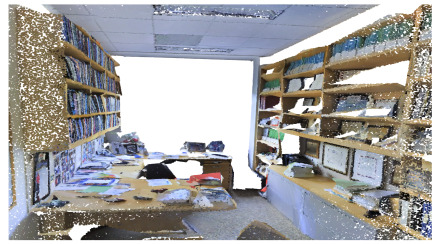
\includegraphics[scale=0.35]{images/s3dis/s3dis_sample_1.jpg}
                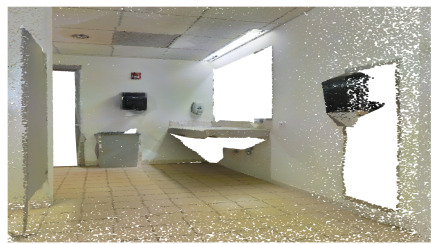
\includegraphics[scale=0.35]{images/s3dis/s3dis_sample_2.jpg}
                \caption{caption}
                \label{fig:s3dis_sample_images}
            \end{figure}
        \end{column}
    \end{columns}
\end{frame}
\begin{frame}{OOD Benchmark datasets}
    \begin{figure}
        \centering
        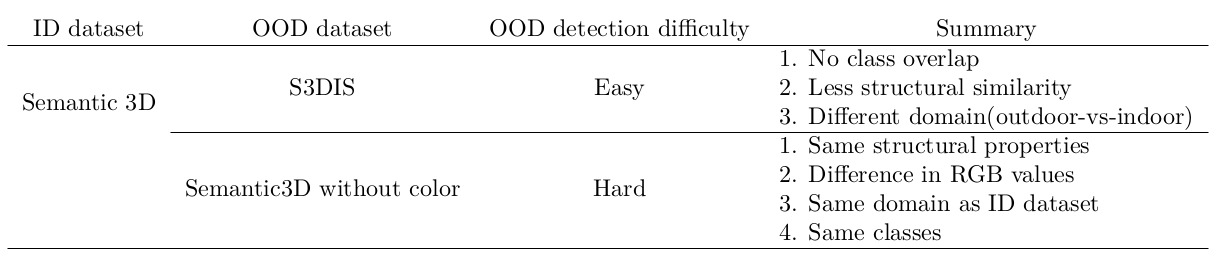
\includegraphics[scale=0.33]{images/benchmark_table.jpg}
        \caption{caption}
        \label{fig:benchmark_table}
    \end{figure}
\end{frame}
\begin{frame}{Ingredients}
    \begin{itemize}
        \item \st{Datasets} - Semantic3D, S3DIS \& Semantic3D w/o colour
        \item 3D Semantic Segmentation model
        \item Uncertainty methods
        \item OOD score methods
    \end{itemize}
\end{frame}
\begin{frame}{RandLA-Net}
    \begin{columns}
        \begin{column}{0.6\textwidth}
            \begin{itemize}
                \item Lightweight, efficient computation, meomry usage and inputs 3D point cloud directly
                \item Random point sampling and local feature aggregation module are most important modules
                \item Local feature aggregation module is subdivided into local spatial encoding, attentive pooling and dilated residual block
                \item Encoder-Decoder style architecture as depicted in Figure\ref{fig:randla_model}
            \end{itemize}
        \end{column}
        \begin{column}{0.4\textwidth}
            \begin{figure}
                \centering
                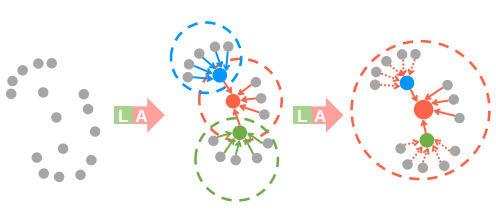
\includegraphics[scale=0.35]{images/randlanet_dires_effect.jpg}
                \caption{caption}
                \label{fig:dires_effect}
            \end{figure}
        \end{column}
    \end{columns}
    
\end{frame}
\begin{frame}{RandLA-Net}
    \begin{figure}
        \centering
        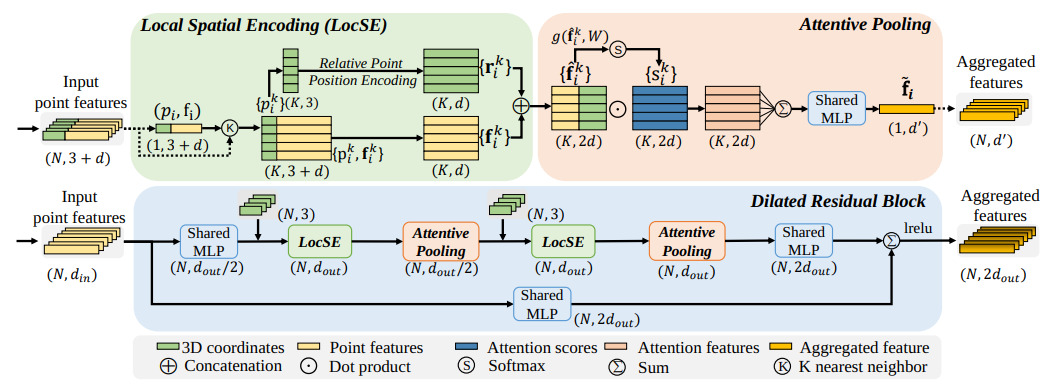
\includegraphics[width = 0.9\textwidth, height=0.37\textheight]{images/randlanet_dires_block.jpg}
        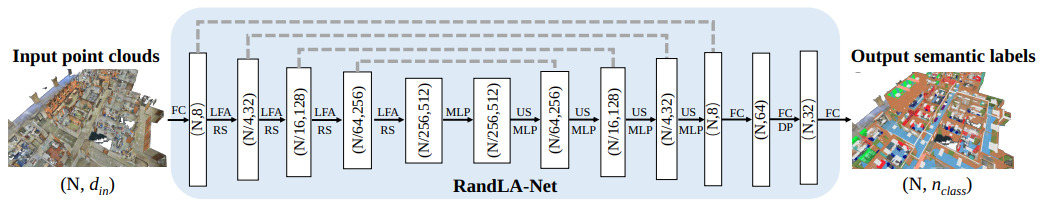
\includegraphics[width = 0.9\textwidth, height=0.37\textheight]{images/randlanet_model.jpg}
        \caption{caption}
        \label{fig:randla_model}
    \end{figure}
\end{frame}
\begin{frame}{Ingredients}
    \begin{itemize}
        \item \st{Datasets} - Semantic3D, S3DIS \& Semantic3D w/o colour
        \item \st{3D Semantic Segmentation model} - RandLA-Net
        \item Uncertainty methods
        \item OOD score methods
    \end{itemize}
\end{frame}
\begin{frame}{Deep Ensembles}
    \begin{columns}
        \begin{column}{0.5\textwidth}
            \begin{itemize}
                \item Ensemble learning technique - train N randomly initialized models with same data
                \item Reulting N predictions are then averged
                \item Perormance boosting along with uncertainty value for a prediction
                \item Requires more computation power
            \end{itemize}
        \end{column}
        \begin{column}{0.5\textwidth}
            \begin{figure}
                \centering
                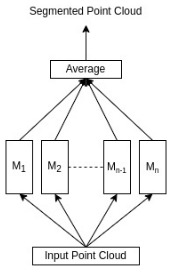
\includegraphics[scale=0.5]{images/deep_ensembles.jpg}
                \caption{caption}
                \label{fig:deep_ensembles_work}    
            \end{figure}
        \end{column}
    \end{columns}
\end{frame}
\begin{frame}{Flipout}
    \begin{columns}
        \begin{column}{0.5\textwidth}
            \begin{itemize}
                \item Introduced as a method to decorrelate gradients in a mini batch of examples
                \item Add independent weight perturbations sampled from a distribution
                \item The output of Flipout versioned neuron is 
                
                \item Train single instance of Flipout versioned network and then perform multiple forward passes for same input
            \end{itemize}
        \end{column}
        \begin{column}{0.5\textwidth}
            \begin{figure}
                \centering
                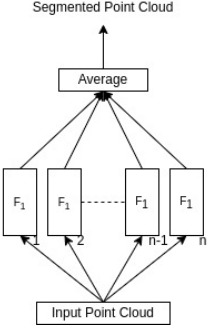
\includegraphics[scale=0.5]{images/flipout.jpg}
                \caption{caption}
                \label{fig:flipout_work}
            \end{figure}
        \end{column}
    \end{columns}
\end{frame}
\begin{frame}{Ingredients}
    \begin{itemize}
        \item \st{Datasets} - Semantic3D, S3DIS \& Semantic3D w/o colour
        \item \st{3D Semantic Segmentation model} - RandLA-Net
        \item \st{Uncertainty methods} - Deep Ensembles \& Flipout
        \item OOD score methods
    \end{itemize}
\end{frame}
\begin{frame}{OOD Score calculation}
    \begin{itemize}
        \item We use the following two methods to generate the OOD scores.
        \item Maximum Softmax Probability
        \begin{itemize}
            \item 
        \end{itemize}
        \item Entropy
        \begin{itemize}
            \item 
        \end{itemize}
    \end{itemize}
\end{frame}
\begin{frame}{Ingredients}
    \begin{itemize}
        \item \st{Datasets} - Semantic3D, S3DIS \& Semantic3D w/o colour
        \item \st{3D Semantic Segmentation model} - RandLA-Net
        \item \st{Uncertainty methods} - Deep Ensembles \& Flipout
        \item \st{OOD score methods} - Maximum Softmax Probability \& Entropy
    \end{itemize}
\end{frame}
%%%%%%%%%%%%%%%%%%%%%%%%%%%%%%%%%%%%%%%%%%%%%%%%%%%%%%%%%%%%%%%%%%%%%%%%%%%%%%%%%%%%%%%%
%%%%%%%%%%%%%%%%%%%%%%%        Experiments          %%%%%%%%%%%%%%%%%%%%%%%%%%%%%%%%%%%%
%%%%%%%%%%%%%%%%%%%%%%%%%%%%%%%%%%%%%%%%%%%%%%%%%%%%%%%%%%%%%%%%%%%%%%%%%%%%%%%%%%%%%%%%
\section{Experiments \& Results}
\begin{frame}{Experiments}
    \begin{itemize}
        \item Semantic3D (ID) vs S3DIS (OOD)
        \begin{itemize}
            \item Deep Ensembles
            \item Flipout
            \item Area Under Receiver Operating Characteristic (AUROC) score comparison
        \end{itemize}
        \item \textcolor{gray}{Semantic3D vs Semantic3D w/o colour}
    \end{itemize}
\end{frame}
\begin{frame}{Semantic3D vs S3DIS - Deep Ensembles}
    \begin{figure}
        \centering
        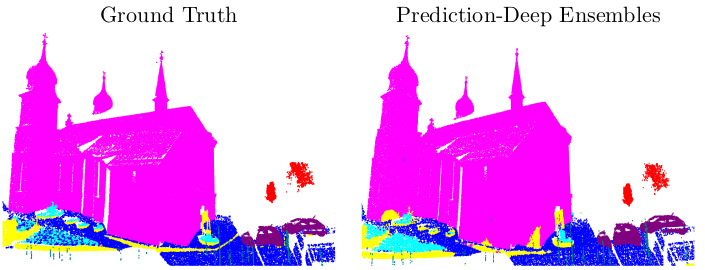
\includegraphics[scale=0.5]{images/sem3d/Sem3d_DE_output.jpg}
        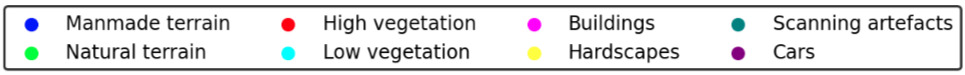
\includegraphics[scale=0.25]{images/legend.jpg}
        \caption{caption}
        \label{fig:sem3d_de_op}
    \end{figure}
\end{frame}
\begin{frame}{Semantic3D vs S3DIS - Deep Ensembles}
    \begin{figure}
        \centering
        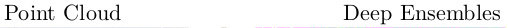
\includegraphics[scale=0.5]{images/s3dis/top_legend_s3dis_DE.jpg}
        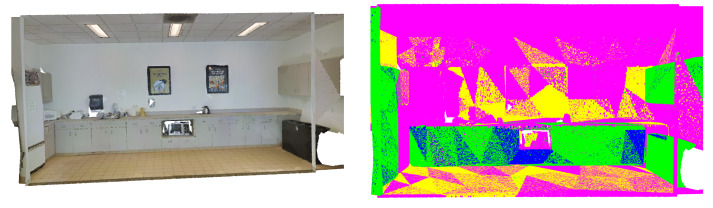
\includegraphics[scale=0.5]{images/s3dis/S3DIS_DE_output.jpg}
        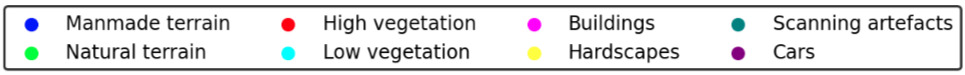
\includegraphics[scale=0.25]{images/legend.jpg}
        \caption{caption}
        \label{fig:s3dis_de_op}
    \end{figure}
\end{frame}
\begin{frame}{Semantic3D vs S3DIS - Deep Ensembles}
    \begin{columns}
        \begin{column}{0.5\textwidth}
            \begin{figure}
                \centering
                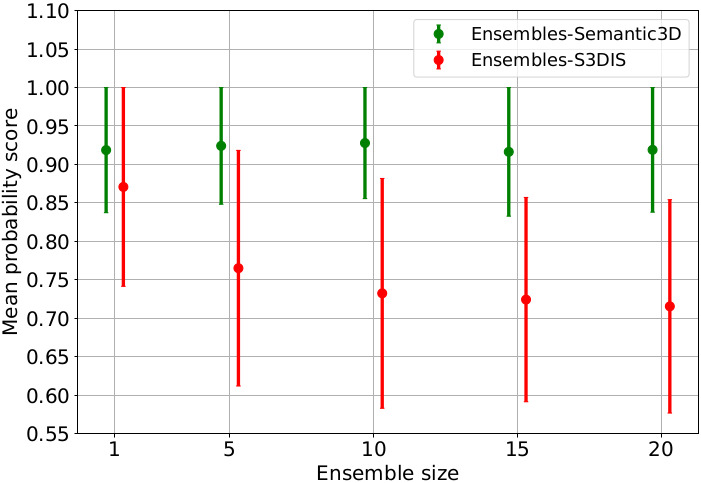
\includegraphics[scale=0.28]{images/ood1/MSP_Mean_OOD1_DE.jpg}
            \end{figure}
        \end{column}
        \begin{column}{0.5\textwidth}
            \begin{figure}
                \centering
                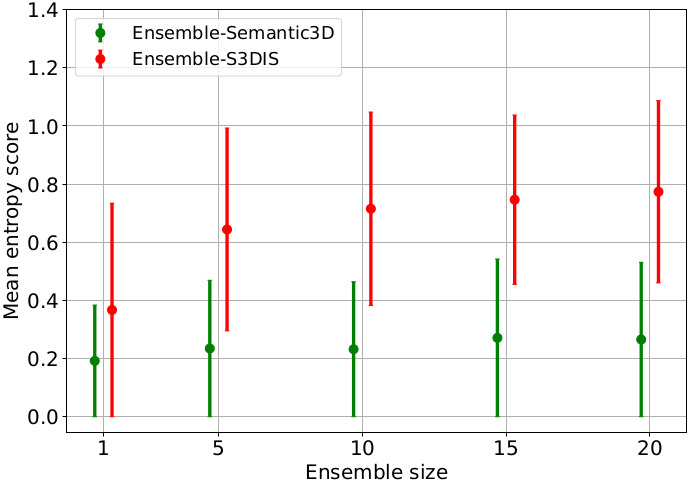
\includegraphics[scale=0.28]{images/ood1/Ent_Mean_OOD1_DE.jpg}
            \end{figure}
        \end{column}
    \end{columns}
\end{frame}

\begin{frame}{Semantic3D vs S3DIS - Flipout}
    \begin{figure}
        \centering
        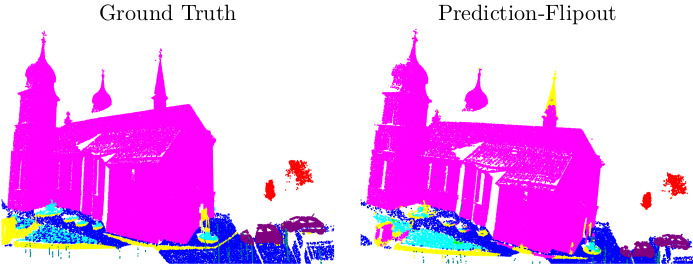
\includegraphics[scale=0.5]{images/sem3d/Sem3d_Fout_op.jpg}
        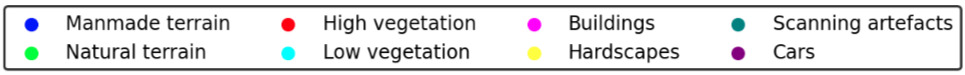
\includegraphics[scale=0.25]{images/legend.jpg}
        \caption{caption}
        \label{fig:sem3d_fout_op}
    \end{figure}
\end{frame}
\begin{frame}{Semantic3D vs S3DIS - Flipout}
    change this image here later dont forget
    \begin{figure}
        \centering
        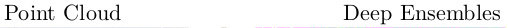
\includegraphics[scale=0.5]{images/s3dis/top_legend_s3dis_DE.jpg}
        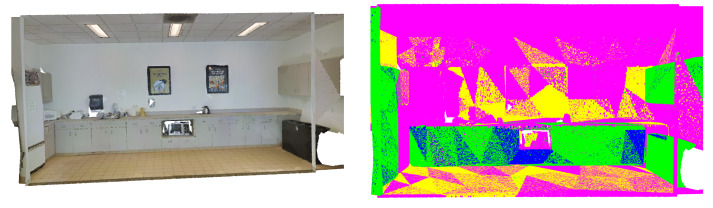
\includegraphics[scale=0.5]{images/s3dis/S3DIS_DE_output.jpg}
        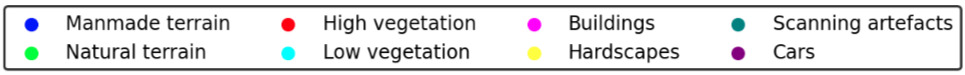
\includegraphics[scale=0.25]{images/legend.jpg}
        \caption{caption}
        \label{fig:s3dis_fout_op}
    \end{figure}
\end{frame}
\begin{frame}{Semantic3D vs S3DIS - Flipout}
    \begin{columns}
        \begin{column}{0.5\textwidth}
            \begin{figure}
                \centering
                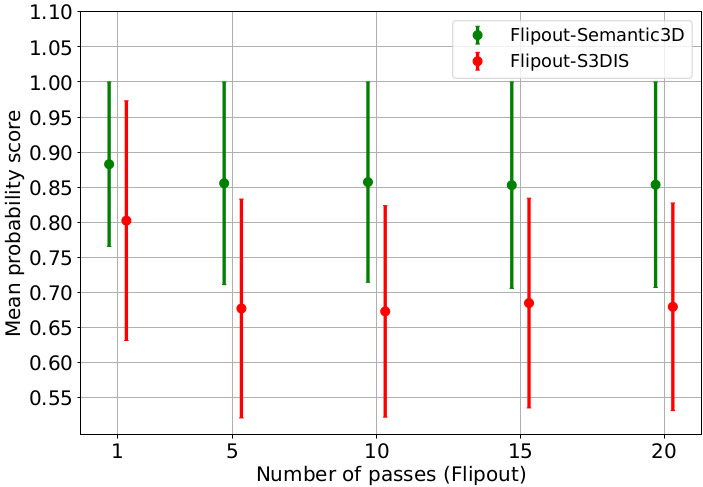
\includegraphics[scale=0.28]{images/ood1/MSP_Mean_OOD1_Fout.jpg}
            \end{figure}
        \end{column}
        \begin{column}{0.5\textwidth}
            \begin{figure}
                \centering
                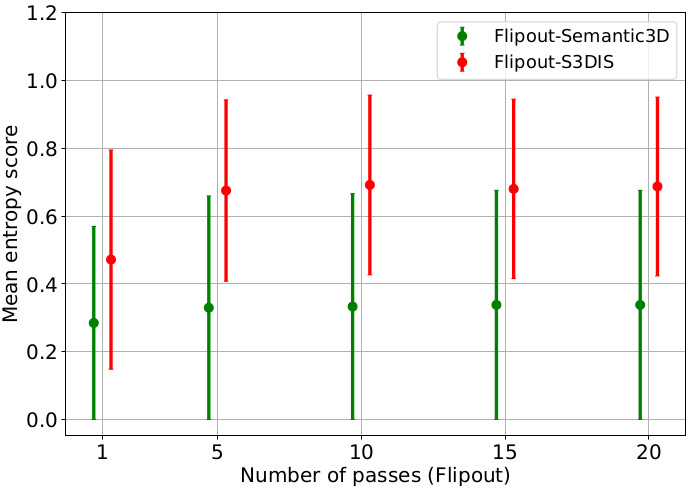
\includegraphics[scale=0.28]{images/ood1/Ent_Mean_OOD1_Fout.jpg}
            \end{figure}
        \end{column}
    \end{columns}
\end{frame}
\begin{frame}{Semantic3D vs S3DIS - AUROC Scores}
    \begin{figure}
        \centering
        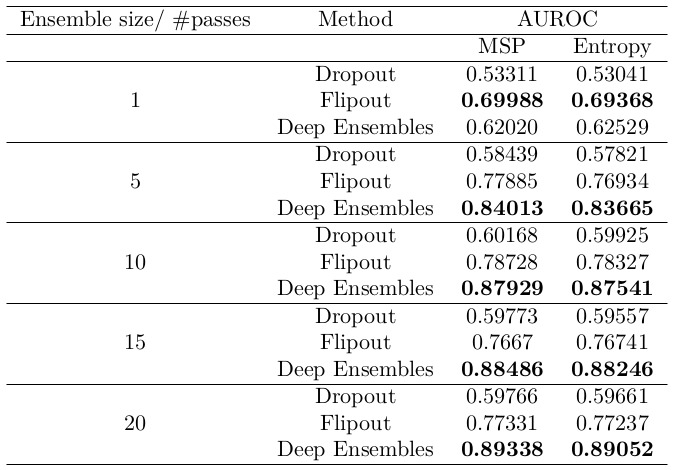
\includegraphics[scale=.35]{images/ood1/AUROC_OOD1_Scores.jpg}
        \caption{caption}
        \label{fig:ood1_AUROC}
    \end{figure}
\end{frame}


%%%%%%%%%%%%%%%%%%%%%%%%%%%%%%%%%%%%%%%%%%%%%%%%%%%%%%%%%%%%%%%%%%%%%%%%%%%%%%%%%%%%%%%%
%%%%%%%%%%%%%%%%%%%%%%%        Experiment2           %%%%%%%%%%%%%%%%%%%%%%%%%%%%%%%%%%%
%%%%%%%%%%%%%%%%%%%%%%%%%%%%%%%%%%%%%%%%%%%%%%%%%%%%%%%%%%%%%%%%%%%%%%%%%%%%%%%%%%%%%%%%
\begin{frame}{Experiments}
    \begin{itemize}
        \item \textcolor{gray}{Semantic3D (ID) vs S3DIS (OOD)}
        
        \item Semantic3D vs Semantic3D w/o colour
        \begin{itemize}
            \item Deep Ensembles
            \item Flipout
            \item Area Under Receiver Operating Characteristic (AUROC) score comparison
        \end{itemize}
    \end{itemize}
\end{frame}
\begin{frame}{Semantic3D colour vs w/o colour - Deep Ensembles}
    \begin{figure}
        \centering
        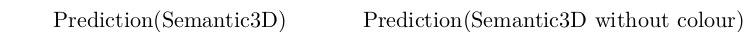
\includegraphics[scale=0.5]{images/ood2/top_legend_ood2.jpg}
        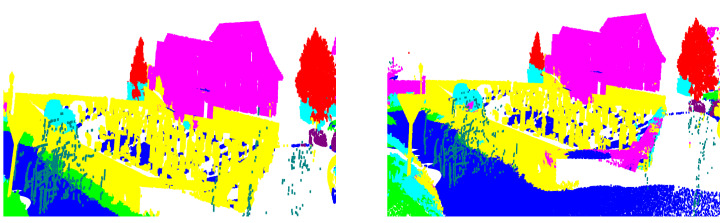
\includegraphics[scale=0.5]{images/ood2/Sem3d_OOD2_DE.jpg}
        \caption{caption}
        \label{fig:DE_ood2_op}
    \end{figure}
\end{frame}
\begin{frame}{Semantic3D colour vs w/o colour - Deep Ensembles}
    \begin{columns}
        \begin{column}{0.5\textwidth}
            \begin{figure}
                \centering
                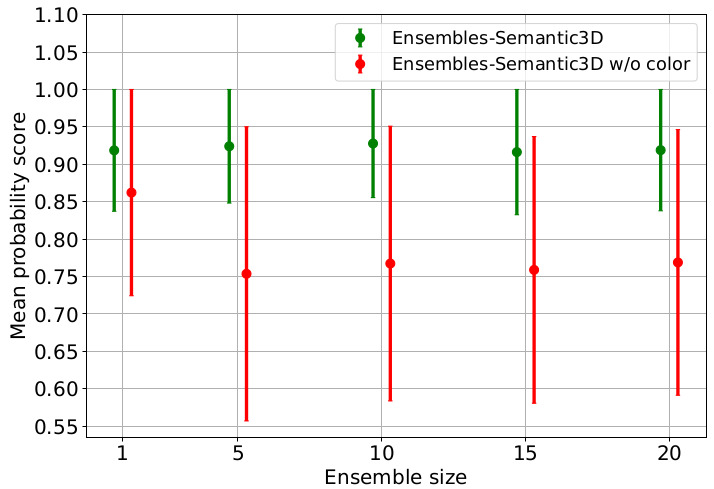
\includegraphics[scale=0.28]{images/ood2/DE_MSP_OOD2.jpg}
            \end{figure}
        \end{column}
        \begin{column}{0.5\textwidth}
            \begin{figure}
                \centering
                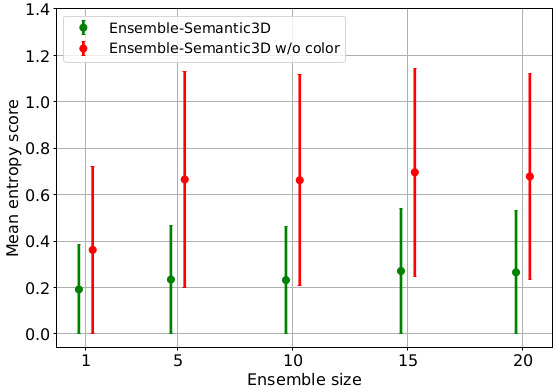
\includegraphics[scale=0.38]{images/ood2/DE_Ent_OOD2.jpg}
            \end{figure}
        \end{column}
    \end{columns}
\end{frame}

%\begin{frame}{Semantic3D colour vs w/o colour - Flipout}
%    \begin{figure}
%        \centering
%        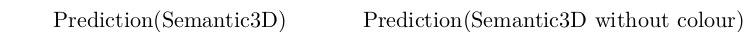
\includegraphics[scale=0.5]{images/ood2/top_legend_ood2.jpg}
%        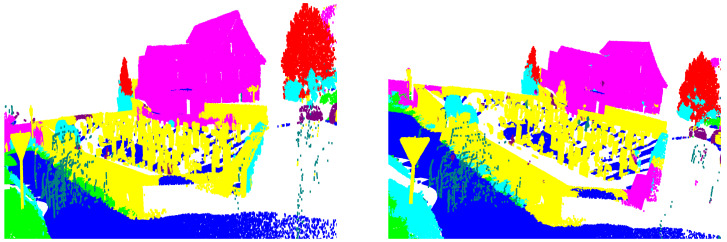
\includegraphics[scale=0.5]{images/ood2/Sem3d_OOD2_Fout.jpg}
%        \caption{caption}
%        \label{fig:Fout_ood2_op}
%    \end{figure}
%\end{frame}
\begin{frame}{Semantic3D colour vs w/o colour - Flipout}
    \begin{columns}
        \begin{column}{0.5\textwidth}
            \begin{figure}
                \centering
                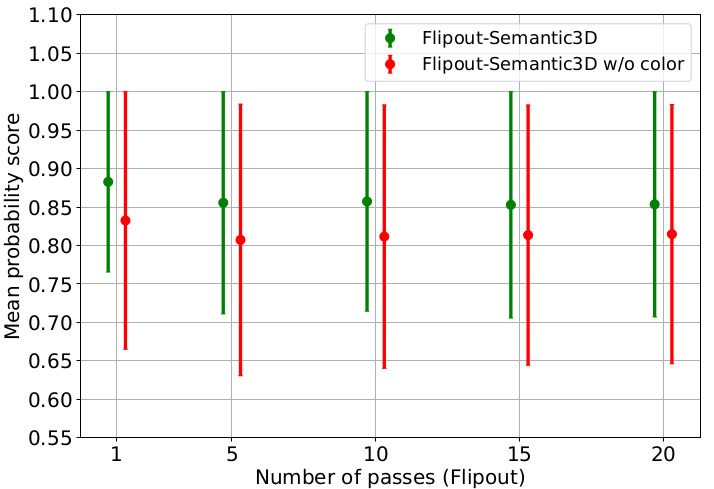
\includegraphics[scale=0.28]{images/ood2/Fout_MSP_OOD2.jpg}
            \end{figure}
        \end{column}
        \begin{column}{0.5\textwidth}
            \begin{figure}
                \centering
                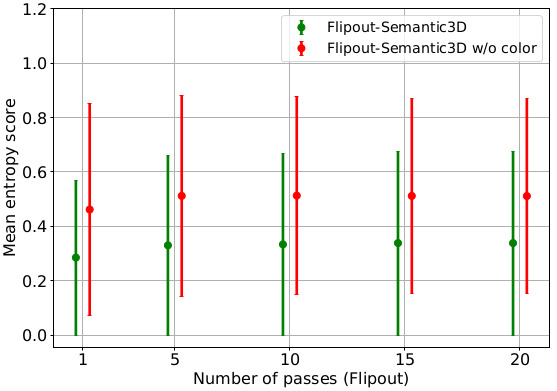
\includegraphics[scale=0.38]{images/ood2/Fout_Ent_OOD2.jpg}
            \end{figure}
        \end{column}
    \end{columns}
\end{frame}

\begin{frame}{Semantic3D colour vs w/o colour - AUROC Scores}
    \begin{figure}
        \centering
        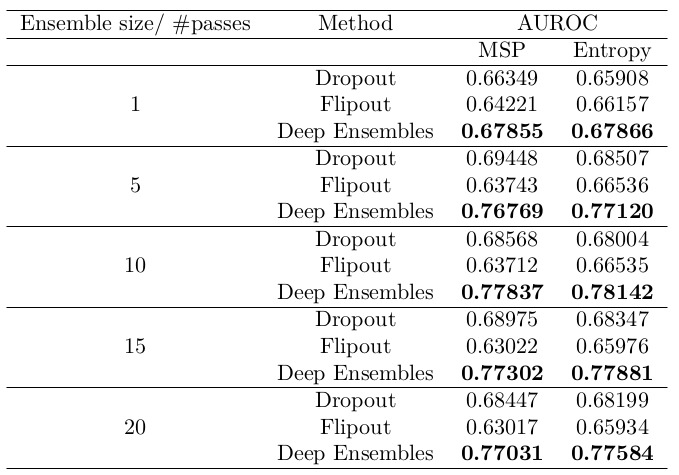
\includegraphics[scale=0.35]{images/ood2/AUROC_OOD2.jpg}
        \caption{caption}
         \label{fig:auroc_scores_ood2}
    \end{figure}
\end{frame}

% Arrange the experiments and explain the results here
%%%%%%%%%%%%%%%%%%%%%%%%%%%%%%%%%%%%%%%%%%%%%%%%%%%%%%%%%%%%%%%%%%%%%%%%%%%%%%%%%%%%%%%%
%%%%%%%%%%%%%%%%%%%%%%%        Conclusion         %%  %%%%%%%%%%%%%%%%%%%%%%%%%%%%%%%%%%
%%%%%%%%%%%%%%%%%%%%%%%%%%%%%%%%%%%%%%%%%%%%%%%%%%%%%%%%%%%%%%%%%%%%%%%%%%%%%%%%%%%%%%%%
\section{Conclusion}
\begin{frame}{Conclusion}
    
\end{frame}
\begin{frame}{Lessons Learned}
    Learning's during the duration of the thesis are
    \begin{enumerate}
        \item Training and evaluation of 3D DNNs are time consuming and resource intensive.
        \item Finding the proper prior for Flipout layers is hard and currently we use brute force to find the best fitting prior.
        \item OOD benchmarking require in depth analysis of datasets like studying the structural similarties in the datasets and also colour spectrum.
        \item LiDAR datasets have large memory requirements especially for the preprocessing and metric computation.
        \item Getting 100\% OOD detection performance is not possible with the post-hoc methods used as some points in the ID dataset also have low probability scores.
    \end{enumerate}
\end{frame}
\begin{frame}{Future Work}
    This thesis can be extended in the following ways.
    \begin{enumerate}
        \item This thesis is limited to only point based models, this can be extended to graph and projection based models.
        \item The datasets involved are only static datasets and this thesis study can be further extended to other type of datasets such as synthetic and sequential datasets.
        \item Since this thesis utilzes post-hoc threshold methods for OOD detection. Other methods such as Mahalanobis distance based OOD detection \cite{lee2018simple_mahalanobis} or MetaSeg \cite{MetaSeg} can be added as an extension to this thesis.
    \end{enumerate}
\end{frame}
%%%%%%%%%%%%%%%%%%%%%%%%%%%%%%%%%%%%%%%%%%%%%%%%%%%%%%%%%%%%%%%%%%%%%%%%%%%%%%%%%%%%%%%%
%%%%%%%%%%%%%%%%%%%%%%%        References%%           %%%%%%%%%%%%%%%%%%%%%%%%%%%%%%%%%%
%%%%%%%%%%%%%%%%%%%%%%%%%%%%%%%%%%%%%%%%%%%%%%%%%%%%%%%%%%%%%%%%%%%%%%%%%%%%%%%%%%%%%%%%

\begin{frame}{References}
    \bibliographystyle{plain}
    \bibliography{bibliography.bib}

\end{frame}
%%%%%%%%%%%%%%%%%%%%%%%%%%%%%%%%%%%%%%%%%%%%%%%%%%%%%%%%%%%%%%%%%%%%%%%%%%%%%%%%%%%%%%%%
%%%%%%%%%%%%%%%%%%%%%%%        Extra slides           %%%%%%%%%%%%%%%%%%%%%%%%%%%%%%%%%%
%%%%%%%%%%%%%%%%%%%%%%%%%%%%%%%%%%%%%%%%%%%%%%%%%%%%%%%%%%%%%%%%%%%%%%%%%%%%%%%%%%%%%%%%

\begin{frame}{What is OOD Detection?}
    \begin{figure}
        \centering
        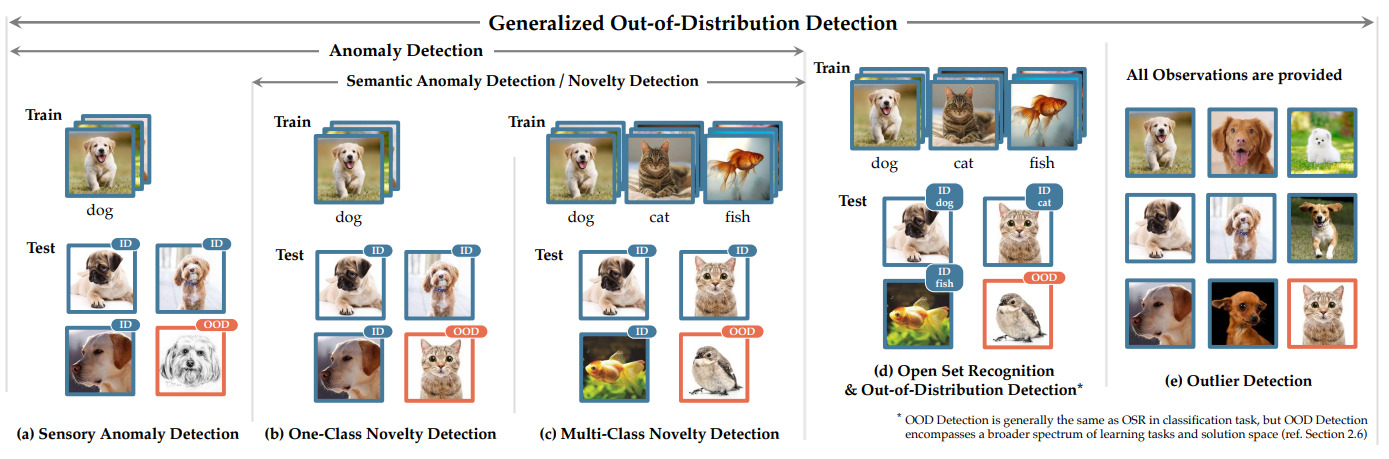
\includegraphics[scale=0.3]{images/OOD_ex_new.jpg}
        \caption{Generalized Out-of-Distribution Detection: A Survey}
        \label{fig:my_label}
    \end{figure}
\end{frame}


\end{document}

